% \iffalse meta-comment
%
% Copyright (C) 2015 by Sven Harder
% -----------------------------------
%
% This file may be distributed and/or modified under the
% conditions of the LaTeX Project Public License, either version 1.3
% of this license or (at your option) any later version.
% The latest version of this license is in:
%
% http://www.latex-project.org/lppl.txt
%
% and version 1.3 or later is part of all distributions of LaTeX
% version 2005/12/01 or later.
%
% \fi
%
% \iffalse
%<package>\NeedsTeXFormat{LaTeX2e}
%<package>\ProvidesPackage{xcookybooky}
%<package> [2015/02/10 v1.5 Easy typesetting (potentially long) recipes with pictures]
%<config>\ProvidesFile{xcookybooky.cfg}
%<config> [2015/02/03 v1.1 'xcookybooky' configuration file]
%
%<*driver>
\documentclass{ltxdoc}
\usepackage[T1]{fontenc}
\usepackage[latin1]{inputenc} 
\usepackage{lmodern}
\usepackage{xcookybooky}
\usepackage{booktabs}
\usepackage{units}
\usepackage{pdfpages}
\usepackage{listings}
\renewcommand{\lstlistingname}{Example}
\renewcommand{\lstlistlistingname}{List of \lstlistingname s}
\lstset
{%
    keywordstyle=\color{blue}\bfseries,
    commentstyle=\ttfamily,
    stringstyle=\ttfamily,
    language=[LaTeX]{TeX},
    breaklines=true,
    captionpos=b,
    gobble=2,
    %morekeywords={unit, bakingtemperature, portion},
}
\EnableCrossrefs
\CodelineIndex
\RecordChanges
\addtolength{\textheight}{-1.5cm}
\addtolength{\oddsidemargin}{0.5cm}
\setcounter{IndexColumns}{2}
\setcounter{GlossaryColumns}{2}
\usepackage{hyperref}
\hypersetup{%
    pdfauthor = {Sven Harder},
    pdftitle = {xcookybooky documentation},
    colorlinks = {true},
    linkcolor = {blue},
    urlcolor = {blue},
    citecolor = {blue},
    filecolor = {blue}
}
\begin{document}
    \DocInput{xcookybooky.dtx}
\end{document}
%</driver>
% \fi
%
% \CheckSum{814}
%
% \CharacterTable
%  {Upper-case    \A\B\C\D\E\F\G\H\I\J\K\L\M\N\O\P\Q\R\S\T\U\V\W\X\Y\Z
%   Lower-case    \a\b\c\d\e\f\g\h\i\j\k\l\m\n\o\p\q\r\s\t\u\v\w\x\y\z
%   Digits        \0\1\2\3\4\5\6\7\8\9
%   Exclamation   \!     Double quote  \"     Hash (number) \#
%   Dollar        \$     Percent       \%     Ampersand     \&
%   Acute accent  \'     Left paren    \(     Right paren   \)
%   Asterisk      \*     Plus          \+     Comma         \,
%   Minus         \-     Point         \.     Solidus       \/
%   Colon         \:     Semicolon     \;     Less than     \<
%   Equals        \=     Greater than  \>     Question mark \?
%   Commercial at \@     Left bracket  \[     Backslash     \\
%   Right bracket \]     Circumflex    \^     Underscore    \_
%   Grave accent  \`     Left brace    \{     Vertical bar  \|
%   Right brace   \}     Tilde         \~}
%
%
% \changes{v1.0}{2011/12/29}{Initial version}
% \changes{v1.1}{2012/04/06}{Load the non-free package 'emerald' per option. Possibility to change the picture width independently from the text columns}
% \changes{v1.2}{2013/03/10}{Better way for displaying the ingredients (tabularx). Thanks to Bartosz Dziubaczyk for developing.}
% \changes{v1.3}{2013/06/04}{Fixed a problem with the default recipe name font. Thanks to V�clav Zeman for reporting. New environment for the ingredients. Thanks to Andreas P�ge for this suggestion.}
% \changes{v1.4}{2015/02/03}{Added two commands for a introduction and recipe suggestions. Additional several hooks are implement in order to insert user-defined text blocks at different places in the recipe. Thanks to Heikki Lehvaslaiho for designing the graphical separator and sending suggestions. Added translations for German, English, French and Spanish.}
% \changes{v1.5}{2015/02/10}{Adding translations for Portuguese and Brazilian. Thanks to Thiago de Melo for submitting.}
%
% \GetFileInfo{xcookybooky.sty}
%
% \DoNotIndex{\#,\$,\%,\&,\@,\\,\{,\},\^,\_,\~,\ ,\"}
% \DoNotIndex{\@ne}
% \DoNotIndex{\advance,\begingroup,\catcode,\closein}
% \DoNotIndex{\closeout,\day,\def,\edef,\else,\empty,\endgroup}
% \DoNotIndex{\begin,\end,\equal,\if,\fi,\ifthenelse,\setcounter,\value,\ifx,\ifnum}
% \DoNotIndex{\RequirePackage}
% \DoNotIndex{\savekeys,\define,\setkeys,\define@key}
%
% \title{The \textsf{xcookybooky} package\thanks{This document
% corresponds to \textsf{xcookybooky}~\fileversion,
% dated \filedate.}}
% \author{Sven Harder \\ \texttt{sven\_one1@gmx.de} \\ \url{https://code.google.com/p/xcookybooky/}}
%
% \maketitle
%
% \begin{abstract}
% This package is made for typesetting recipes. You simply enter ingredients, preparation steps and get a beautiful recipe page. It is also possible to enter two pictures, which are displayed above the name of the recipe. Another option is to write a introduction, several suggestions and s hint, which is displayed at the bottom of the page.
% \end{abstract}
%
% \vspace{3em}
%
% \PrintChanges
%
% \newpage
% \tableofcontents
% \newpage
%
% \section{Introduction}
%
% It all begin in 2011 when I wanted to make a cookbook with \LaTeX. Thus I was looking for recipe templates and found the \texttt{cookybooky} package by J�rgen Gilg (\url{http://www.ctan.org/pkg/cookybooky}). It looks very good, but I was unable to compile it (e.g. I haven't got the Lucida fonts). Also there are some packages which have to be downloaded by hand, because there are not available at CTAN. Other handicaps are the missing possibility to create a PDF-file directly and a recipe cannot be longer than a single page. So decided to take a look at the code. Step by step I replaced all critical parts. Finally the code is nearly complete different from the original and now it is possible to create beautiful designed recipes much easier (at least in my opinion).
% 
% Please note that there is no compatibility between xcookybooky and cookybooky, even the name is associating it. I chose the name, because I was was inspired by the layout.
%
%
% \section{Usage}
% In this section the most important macros are explained. After this you should be able to insert recipes. For more details take a look at the implementation in section~\ref{sec:implementation}. Afterwards some macros are shown, which allows you to modify the design (e.g. colors, headlines).
%
% \subsection{Main}
% This commands are commonly used for typesetting recipes. For more details take a look at the implementation in section~\ref{sec:implementation}. You can also investigate the examples and the configuration file.
%
% \DescribeEnv{recipe}
% The \texttt{recipe} environment is used to insert recipes. Each recipe is included in a single enviroment. It is necessary to enter the name of the recipe. Besides it is possible to insert also the recipetime, the portions, the calory content and the source (where you get this recipe).
% 
% \begin{lstlisting}[caption={Recipe Environment}]
% \begin{recipe}
% [% 
%     preparationtime = {\unit[1]{h}},
%     bakingtime={\unit[1]{h}},
%     bakingtemperature={\protect\bakingtemperature{fanoven=\unit[230]{�C}}},
%     portion = {\portion{5-6}},
%     calory={\unit[3]{kJ}},
%     source = {Somebody you used know}
% ]
% {Test Recipe}
% ...
% \end{recipe}
% \end{lstlisting}
%
% \DescribeMacro{\graph}
% It is possible to set two pictures by using the macro \texttt{graph}. They are displayed at the top of the page and therefore above all other content. If no pictures are set, the space is used by the other content. The \texttt{big} picture should be larger than the \texttt{small} picture of course. The width of both graphics can be adapt to your needs by applying the command \texttt{setRecipeLengths}.
%
% \begin{lstlisting}[caption={Graph Command (simple)}]
% \graph{
%     small = strawberry,
%     big = strawberrycake
% }
% \end{lstlisting}
%
% Another possibility is shown in the following example. It is recommended if you only want to change the widths of the pictures for one recipe, because these values are one only used for one recipe. If you want to changed it for all recipes use \texttt{setRecipeLengths}.
%
% \begin{lstlisting}[caption={Graph Command (extended)}]
% \graph{
%     small = strawberry,
%     smallpicturewidth = 0.3\textwidth,
%     big = strawberrycake,
%     bigpicturewidth = 0.6\textwidth,
% }
% \end{lstlisting}
%
% \DescribeMacro{\ingredients}
% Here the ingredients of your recipe are set. They should be entered by number (unit) \& ingredient. If the unit is a SI-Unit, it looks better if you use the \texttt{units} package instead of a blank.
% Since the version 1.2 there is only one possibility to enter ingredients, which is shown in the example. Note that a overlong ingredient will automatically create a line break.
%
% \begin{lstlisting}[caption={Ingredients Command}]
% \ingredients{
%     2 bar & Dark Chocolate (above \unit[70]{\%})\\
%     3 & Eggs\\
%     \unit[200]{ml} & Cream\\
%     \unit[40]{g} & Sugar\\
%     \unit[50]{g} & Butter
% }
% \end{lstlisting}
%
% In the versions up to 1.1 there was also a method to enter ingredients with three columns. Due to the substitution of \texttt{tabular} with \texttt{tabulary} I decided that the three columns method is no longer supported, because it would mean a lot of work. This method has also the drawback it needs more space and in my opinion it also looks ugly.
% If you are using the three columns solution there are two options:
% \begin{enumerate}
%   \item Use the version 1.1 of this package, which can be found at \url{https://code.google.com/p/xcookybooky/}
%   \item Redefine the concerning command in your latex file or in the configuration file 
% \end{enumerate}
% 
% \DescribeMacro{\preparation}
% The preparation steps are inserted by this macro. Every step is written after \texttt{step} command. This is necessarry for the numeration. Since version 1.4 it is allowed to use blank lines to create passages. 
%
% \begin{lstlisting}[caption={Preparation Command}]
% \preparation{
%     \step This is the first step for cooking a brilliant meal.
%     \step The second step follows...
%     \step and so on
%     \step Enjoy your meal! 
% }
% \end{lstlisting}
%
% If you don't like the step number, you can either redefine it or simply use an enumeration as demonstrated in the next example.
% \begin{lstlisting}[caption={Preparation Command with Enumeration}]
% \preparation{
%     \begin{enumerate}
%         \item This is the first step for cooking a brilliant meal.
%         \item The second step follows...
%         \item and so on
%         \item Enjoy your meal! 
%     \end{enumerate}
% }
% \end{lstlisting}
%
%
% \subsection{Advanced}
% 
% \DescribeMacro{\introduction}
% The \texttt{introduction} macro can be used for inserting an introduction before the preparation and ingredients part. It has a frame and the text can contain blank lines to create passages.
%
% \begin{lstlisting}[caption={Introduction Command}]
% \introduction{%
%     This text block can contain an introduction to the recipe.
% }
% \end{lstlisting}
% 
% \DescribeMacro{\suggestion}
% This command is displayed after the ingredients and preparation part of the recipe. It is expandable so that you can insert multiple suggestions. The optional parameter can be used to set a headline.
% \begin{lstlisting}[caption={Suggestion Command}]
% \suggestion{%
%     Another possibility to insert additional information to the recipe.
% }
% % \suggestion[Headline]{%
%     Another possibility to insert additional information to the recipe.
% }
% \end{lstlisting}
%
% \subsection{Support Commands}
% \DescribeMacro{\portion}
% This macro is intented as an interface for an equal formating of portions entries. For this it can be easily modified. You just have to renew this command.
% \begin{lstlisting}[caption={Portion Command}]
% \portion{5}
% \portion[People]{5}
% \end{lstlisting}
%
% \DescribeMacro{\bakingtemperature}
% This macro allows you to enter some bakingtemperatures. If you do not like the order of the temperatures you can change them by redefining the command. The temperatures are inserted as key/value pairs as known from the \texttt{xkeyval} package.
%
% \begin{lstlisting}[caption={Baking Temperature Command}]
% \begin{recipe}
% [
%     bakingtemperature={\protect\bakingtemperature{
%         fanoven=\unit[230]{�C},
%         topbottomheat=\unit[195]{�C},
%         topheat=\unit[195]{�C},
%         bottomheat, gasstove=Level 2}
%     }
% ]{Test Recipe}
% \end{recipe}
% \end{lstlisting}
%
%
% \subsection{Modify Design}
% The following macros can be used outside the recipe environment to choose your personal color etc.
%
% \DescribeMacro{\setRecipeColors}
% If you want to change the default colors, you can use \texttt{setRecipeColors}. The colors are set by <key~=~value> as known by the \texttt{xkeyval} package. The names of colors can be found in table \ref{tbl:colormanagement}. 
% \begin{table}[htbp]
%     \centering
%     \begin{tabular}{rcl}
%         \textbf{Key}    & \textbf{Default Value} & \textbf{Description} \\
%         \toprule
%         recipename      & DarkGreen & recipe name \\
%         intro           & black     & introduction \\
%         ing             & DarkGray  & ingredients (text) \\
%         inghead         & DarkGray  & headline of the ingredients \\
%         prep            & black     & preparation (text) \\
%         prephead        & black     & headline of the preparation \\
%         suggestion      & black     & suggestions (text) \\
%         suggestionhead  & black     & headline of suggestions\\
%         separationgraph & black     & graphical separator \\
%         hint            & red       & hint (text) \\
%         hinthead        & red       & headline of the hint \\
%         hintline        & red       & lines leftside the hint text (cross) \\
%         numeration      & red       & numeration of the preparation steps \\ 
%     \end{tabular}
%     \caption{Color Management}
%     \label{tbl:colormanagement}
% \end{table}
% New colors can be easiliy defined by the \texttt{xcolor} package as shown the example below.
% 
% \begin{lstlisting}[caption={Setting Recipe Colors Command}]
% \definecolor{webgreen}{rgb}{0,.5,0}
%
% \setRecipeColors{
%     recipename = webgreen,
%     ing = blue,
%     numeration = black,    
% }
% \end{lstlisting}
%
% \DescribeMacro{\setRecipeLengths}
% By using the command \texttt{setRecipeLengths} it is possible to change the (default) values for the picture widths and the text column widths. In the table~\ref{tbl:recipelengths} all implemented keys are listed.
% \begin{table}[htbp]
%     \centering
%     \begin{tabular}{rl}
%         \textbf{Key}    & \textbf{Description} \\
%         \toprule
%         pictureheight      & height of both pictures \\
%         bigpicturewidth    & width of the bigger picture \\
%         smallpicturewidth  & width of the smaller picture \\
%         introductionwidth  & width of introduction \\
%         preparationwidth   & width of preparation \\
%         ingredientswidth   & width of ingredients
%     \end{tabular}
%     \caption{Recipe Lengths}
%     \label{tbl:recipelengths}
% \end{table}
% 
% \begin{lstlisting}[caption={Setting Recipe Lengths Command}]
% \setRecipeLengths{
%     preparationwidth = 0.5\textwidth,
%     ingredientswidth = 0.4\textwidth,
% }
% \end{lstlisting}
%
% \DescribeMacro{\setRecipeSizes}
% The macro \texttt{setRecipeSizes} enables you to modify the font size of many parts of the recipe. The sizes are inserted by <key~=~value> (\texttt{xkeyval}). All supported keys can be found in the following table~\ref{tbl:sizemanagement}.
% \begin{table}[htbp]
%     \centering
%     \begin{tabular}{rl}
%         \textbf{Key}    & \textbf{Description} \\
%         \toprule
%         recipename    & font size of recipe name \\
%         intro         & font size of introduction (text) \\
%         ing           & font size of ingredients (text) \\
%         inghead       & font size of headline of ingredients \\
%         prephead      & font size of headline of preparation \\
%         suggestion    & font size of suggestion (text) \\
%         hint          & font size of hint (text) \\
%         hinthead      & font size of headline of hint
%     \end{tabular}
%     \caption{Font Size Management}
%     \label{tbl:sizemanagement}
% \end{table}
%
% \begin{lstlisting}[caption={Setting Recipe Sizes Command}]
% \setRecipeSizes{
%     recipename = \fontsize{25pt}{30pt},
%     ing = \normalsize,
%     hinthead = \Large
% }
% \end{lstlisting}
%
% \DescribeMacro{\setRecipenameFont}
% The name of recipe is only displayed with a handwritten font, if the corresponding option is selected. See section~\ref{sec:options} for details. In my opinion it looks much better than a standard font. But if you want to change it you can use this macro. A well-arranged list of fonts can be found at \url{http://www.tug.dk/FontCatalogue/}. The four parameters are font name,font encoding, font series and font shape. The size is changed by \texttt{setRecipeSizes}. The following example shows a bunch of interesting fonts, which you should try out.
%
% \begin{lstlisting}[caption={Setting Recipename Font Command (package \texttt{pbsi})}]
% \setRecipenameFont{cmr}{T1}{m}{n} % probably the default setting
% \usepackage{pbsi}
% \setRecipenameFont{pbsi}{T1}{xl}{n}
% \end{lstlisting}
% \begin{lstlisting}[caption={Setting Recipename Font Command (package \texttt{emerald})}]
% \usepackage{emerald}
% \setRecipenameFont{fau}{T1}{m}{n}
% \setRecipenameFont{fwb}{T1}{m}{n}
% \setRecipenameFont{fjd}{T1}{m}{n} % default by option handwritten
% \end{lstlisting}
%
%
% \subsection{Translation}
% \DescribeMacro{\setHeadlines}
% The command \texttt{setHeadlines} allows to modify the (translated) headlines. This is also needed for translations, if the used language is not supported yet. If you have improvements for a translation or created a new one, feel free to send me a e-mail. 
% The headlines are also inserted in <key~=~value> form. All possible key are described in table~\ref{tbl:headlines}.
% \begin{table}[htbp]
%     \centering
%     \begin{tabulary}{0.75\textwidth}{rcL}
%         \textbf{Key} & \textbf{Graphic} & \textbf{Description} \\
%         \toprule
%             inghead           & no  & Headline of ingredients \\
%             prephead          & no  & Headline of preparation \\
%             hinthead          & no  & Headline of hint \\
%             continuationhead  & no  & Text at the top of the second page of a recipe \\
%             continuationfoot  & no  & Text at the bottom of the first page, if the recipe is longer than one page \\
%             preparationtime   & yes & \\
%             bakingtime        & yes & \\
%             bakingtemperature & yes & \\
%             portion           & yes & \\
%             portionvalue      & no  & Unit for the portions \\
%             calory            & no  & Text for the calorific value \\
%             source            & yes & \\
%     \end{tabulary}
%     \caption{Recipe Headlines}
%     \label{tbl:headlines}
% \end{table}
%
% \begin{lstlisting}[caption={Setting Headlines Command}]
% \setHeadlines{
%     inghead = Ingredients,
%     hinthead = Straight Tip,
%     continuationhead = Continuation \dots,
% }
% \end{lstlisting}
%
%
% \subsection{Options}
% \label{sec:options}
% This package provides three options which are explained in the following.
% \begin{samepage}
% \begin{itemize}
%     \item \textbf{handwritten} This option requires the non-free package \texttt{emerald} and can only be used if your are not using TeX Live.
%     \item \textbf{nowarnings} This options tries to eliminate all nasty warnings. Only important and interesting warnings are logged. This is in my opinion a good choice because the package \texttt{wrapfigure} generates a lot of warnings, see section \ref{sec:knownissues}.
%     \item \textbf{myconfig} If you are using this package often or want to keep your main file 'clean' you can define your modfications in the configuration file. If you submit this option the file will be loaded otherwise \textbf{not}.
% \end{itemize}
% \end{samepage}
%
% \subsection{Background graphic}
% \label{sec:background}
% Inside this package there is only the option to set a background picture using the \texttt{setBackgroundPicture} macro. For creating transparent backgrounds I recommand \textbf{Inkscape}\footnote{http://inkscape.org/}. You just have to import a picture and reduce the opacity of the picture (I prefer \unit[22]{\%}). The possible options for the orientation are: 
% \vspace{-1em}
% \begin{itemize}
%     \item default
%     \item pagecenter
%     \item textcenter
%     \item stockcenter
% \end{itemize}
% These orientations can be modified by using the \texttt{x} and \texttt{y} option. This is demonstrated in the following example.
%
% \begin{lstlisting}[caption={Background Picture Command}]
% \setBackgroundPicture
% [%
%     x = 2cm,
%     y = -1cm,
%     width=\paperwidth-3cm,
%     height,
%     orientation=pagecenter
% ]{pic/bg_transparent} % filepath
% \end{lstlisting} 
%
% \newpage
% \IfFileExists{example/example.pdf}
% {
% \section{Example}
% \begin{minipage}{\textheight}
% \includepdf[pages={2}, scale=0.86]{example/example.pdf}
% \end{minipage}
% \newpage
% }{}
%
% \section{Troubleshooting}
% \subsection{MiKTeX}
% If you have problems with the used fonts (e.g. \texttt{cookingsymbols}) it might be necessary to refresh the database of MiKTeX.
%
% \subsection{TeX Live}
% If you are using this distribution you may should not use the option \texttt{handwritten}, because this option load the font package \texttt{emerald}.
% This package is non-free and therefore not available in TeX Live.
%
% \section{Bugs}
% If you found a bug, which is not described in the following section, feel free to write me an email. It can be found at the titlepage. Alternatively you can visit \url{https://code.google.com/p/xcookybooky/} and report the issue. All reported problems are registered there.
%
% \subsection{Known Issues}
% \label{sec:knownissues}
% The \texttt{wrapfig} package has some problems with enumerations and the \texttt{lettrine} package. This is the reason, why some warnings are generated by compiling (the example), if do not use the package option \textbf{nowarnings}. But nevertheless the results look quite well, so I decided to ignore this issue.
% By using \texttt{wrapfig} it is not possible to switch ingredients and preparation (the result looks really ugly). This is the reason, why the layout is not changed when setting the \texttt{twoside} option in the document class. I also tried \texttt{parcolumns} and \texttt{parallel}, but the results were disappointing. If you want to use this feature, you have to use \texttt{cookybooky}.
%
% Another limitation is the length of the ingredients. The maximum length is one page, because the \texttt{wrapfigure} package does not work with \texttt{longtable}. As a result no pagebreak in the ingredients is possible.
% \StopEventually{\PrintIndex}
%
%
% \newpage
%
% \section{Implementation}
% \label{sec:implementation}
% Let's have a look at the implementation.
%
% \subsection{Options}
% \texttt{xcookybooky} provides three options as explained in section~\ref{sec:options}. You can use the option \texttt{myconfig} to load your personal configuration (file). See section \ref{sec:configuration} for details.
%    \begin{macrocode}
%<*package>
\newif\ifHandwrittenFont@required
\HandwrittenFont@requiredfalse
\DeclareOption{handwritten}
{% displays the recipename in a handwitten font
    \HandwrittenFont@requiredtrue           
    \AtEndOfPackage{
        \setRecipeSizes{recipename = \fontsize{25pt}{30pt}}
        \setRecipenameFont{fjd}{T1}{m}{n}
    }
}
\DeclareOption{nowarnings}
{% tries to eliminate nasty warnings
    \AtEndOfPackage{
        \def\WF@conflict{}
        %\def\@fancywarning#1{}
    }
}
\DeclareOption{myconfig}
{% load personal configuration
    \AtEndOfPackage{
        \InputIfFileExists{xcookybooky.cfg}
        {\PackageInfo{xcookybooky}{inputting 'xcookybooky.cfg'}}
        {\PackageWarning{xcookybooky}{cannot find the configuration file 'xcookybooky.cfg'}}
    }
}
\ProcessOptions\relax

%    \end{macrocode}
%
% \subsection{Required Packages}
%  All needed packages are available at CTAN and as far as I know no general driver limitation are given.
%    \begin{macrocode}
\RequirePackage{tikz}                        % for creating the lines for the hint
\RequirePackage{graphicx}
\RequirePackage{xcolor}
\RequirePackage[clock, misc, weather]{ifsym} % Symbol package e.g. \Interval, \Wecker etc
\RequirePackage{cookingsymbols}              % Cookings symbols e.g. \Oven, \Dish etc
\ifHandwrittenFont@required
    \RequirePackage{emerald}                 % Handwritten Fonts
\fi
\RequirePackage{wrapfig}                     % To wrap the tabular with the ingredients

\RequirePackage{iflang}                      % detecting the language
\RequirePackage{ifthen}
\RequirePackage{xkeyval}
\RequirePackage{lettrine}                    % numbering the preparation steps
\RequirePackage{fancyhdr}
\RequirePackage{units}
\RequirePackage{eso-pic}                     % for background pictures
\RequirePackage{picture}                     % for modfifying the position of the bg pictures
\RequirePackage{tabulary}                    % line breaks in tabular
\RequirePackage{framed}                      % frame for the introduction

%    \end{macrocode}
%
% \subsection{Page Layout}
% This will set up the page. It is optimized for the document class \texttt{article}. If you use an other class you probably have to modify this.
%
% \textbf{Note:} I tried to use the KOMA class \texttt{scrartcl}, but unfortunately some strange effects occured.
%    \begin{macrocode}
\setlength{\parindent}{0cm}
\setlength{\parskip}{2ex plus 0.5ex}

\setlength{\textwidth}{15.5cm}
\setlength{\textheight}{24.0cm}
\setlength{\topmargin}{-0.8cm}
\setlength{\headheight}{14pt} %0cm
\setlength{\headsep}{1cm}
\setlength{\topskip}{0cm}
\setlength{\footskip}{1.4cm}
\setlength{\evensidemargin}{-0.5cm}
\setlength{\oddsidemargin}{0.5cm}
\setlength{\voffset}{0cm}
\setlength{\hoffset}{0cm}
\setcounter{secnumdepth}{2} % subsubsections not numbered
\setcounter{tocdepth}{3}    % subsubsections in the .toc file

%    \end{macrocode}
%
% \begin{macro}{\recipesection}
% The macro \texttt{recipesection} allows to modify the entry in the table of contents.
%
% \textbf{Note:} If you modify the macro you may change the two upper lines as well.
%    \begin{macrocode}
\newcommand*{\recipesection}[2][]
{%
    \subsubsection[#1]{#2}
}

%    \end{macrocode}
% \end{macro}
%
% \subsection{Color Management}
% At first the used non-standard colors must be defined.
%    \begin{macrocode}
\providecolor{DarkGreen}{rgb}{0,.5,0}
\providecolor{DarkBlue}{rgb}{0, 0, 0.7}
\providecolor{DarkGray}{rgb}{0.23, 0.23, 0.23}

%    \end{macrocode}
% Below the (default) colors are defined using the \texttt{xkeyval} package.
%    \begin{macrocode}
\define@key{colorManagement}{recipename}[DarkGreen]{\def\xcb@color@recipename{#1}}
\define@key{colorManagement}{intro}[black]{\def\xcb@color@intro{#1}}
\define@key{colorManagement}{ing}[DarkGray]{\def\xcb@color@ing{#1}}
\define@key{colorManagement}{inghead}[DarkGray]{\def\xcb@color@inghead{#1}}
\define@key{colorManagement}{prep}[black]{\def\xcb@color@prep{#1}}
\define@key{colorManagement}{prephead}[black]{\def\xcb@color@prephead{#1}}
\define@key{colorManagement}{suggestion}[black]{\def\xcb@color@suggestion{#1}}
\define@key{colorManagement}{suggestionhead}[black]{\def\xcb@color@suggestionhead{#1}}
\define@key{colorManagement}{separationgraph}[black]{\def\xcb@color@separationgraph{#1}}
\define@key{colorManagement}{hint}[black]{\def\xcb@color@hint{#1}}
\define@key{colorManagement}{hinthead}[red]{\def\xcb@color@hinthead{#1}}
\define@key{colorManagement}{hintline}[red]{\def\xcb@color@hintline{#1}}
\define@key{colorManagement}{numeration}[red]{\def\xcb@color@numeration{#1}}
\savekeys{colorManagement}
{%
    recipename,      % color of recipename
    intro,           % color of introduction (text)
    ing,             % color of ingredients (text)
    inghead,         % color of headline of ingredients
    prep,            % color of preparation (text)
    prephead,        % color of headline of preparation
    suggestion,      % color of suggestions (text)
    suggestionhead,  % color of headline of suggestion
    separationgraph, % color of graphical separator
    hint,            % color of hint (text)
    hinthead,        % color of headline of hint
    hintline,        % color of lines of hint
    numeration       % color of numeration (preparation)
}

%    \end{macrocode}
%
% \begin{macro}{\setRecipeColors}
% The parameter are set in the form "key~=~value" as known by the \texttt{xkeyval} package.
%    \begin{macrocode}
\newcommand*{\setRecipeColors}[1]
{%
    \setkeys{colorManagement}{#1}
}

%    \end{macrocode}
% \end{macro}
%
% This is the initialisation of all required recipe colors.
%    \begin{macrocode}
\setRecipeColors
{% initialisation
    recipename,
    intro,
    ing,
    inghead,
    prep,
    prephead,
    suggestion,
    suggestionhead,
    separationgraph,
    hint,
    hinthead,
    hintline,
    numeration
}

%    \end{macrocode}
% \subsection{Size Management}
% Below the (default) font sizes of the recipe are defined.
%    \begin{macrocode}
\define@key{sizeManagement}{recipename}[\fontsize{25pt}{30pt}]{\def\xcb@fontsize@recipename{#1}}
\define@key{sizeManagement}{intro}[\normalsize]{\def\xcb@fontsize@intro{#1}}
\define@key{sizeManagement}{ing}[\normalsize]{\def\xcb@fontsize@ing{#1}}
\define@key{sizeManagement}{inghead}[\normalsize]{\def\xcb@fontsize@inghead{#1}}
\define@key{sizeManagement}{prep}[\normalsize]{\def\xcb@fontsize@prep{#1}}
\define@key{sizeManagement}{prephead}[\normalsize]{\def\xcb@fontsize@prephead{#1}}
\define@key{sizeManagement}{suggestion}[\normalsize]{\def\xcb@fontsize@suggestion{#1}}
\define@key{sizeManagement}{hint}[\normalsize]{\def\xcb@fontsize@hint{#1}}
\define@key{sizeManagement}{hinthead}[\Large]{\def\xcb@fontsize@hinthead{#1}}
\savekeys{sizeManagement}
{
    recipename,    % font size of recipe name
    intro,         % font size of introduction (text)
    ing,           % font size of ingredients (text)
    inghead,       % font size of headline of ingredients
    prep,          % font size of preparation (text)
    prephead,      % font size of headline of preparation
    suggestion,    % font size of suggestion (text)
    hint,          % font size of hint (text)
    hinthead       % font size of headline of hint
}

%    \end{macrocode}
%
% \begin{macro}{\setRecipeSizes}
% The parameter are set in the form "key~=~value" as known by the \texttt{xkeyval} package.
%    \begin{macrocode}
\newcommand*{\setRecipeSizes}[1]
{%
    \setkeys{sizeManagement}{#1}
}

%    \end{macrocode}
% \end{macro}
% This is the initialisation of all required recipe sizes.
%    \begin{macrocode}
\setRecipeSizes
{% initialisation
    recipename,
    intro,
    ing,
    inghead,
    prep,
    prephead,
    suggestion,
    hint,
    hinthead
}

%    \end{macrocode}
%
% \subsection{Recipe Font}
%
% \begin{macro}{\setRecipenameFont}
% This macro sets the font for the name of the recipe. You have to insert the font family, font encoding, font series and font shape. The size is set by the command \texttt{sizeManagement}.
%    \begin{macrocode}
%% Handwritten fonts: hlce, pbsi, hlcw, fjd, fau
%% Other fonts: fwb
\newcommand*{\setRecipenameFont}[4]
{% sets the font for the recipename
    \def\xcb@font@recipename
    {
        \fontfamily{#1}
        \fontencoding{#2}
        \fontseries{#3} %x1
        \fontshape{#4}
        \xcb@fontsize@recipename
        \selectfont
    }
}
%    \end{macrocode}
% \end{macro}
%
% This is the initialisation of the font of the recipename. The default is set to the system default settings to support as many \LaTeX{} distributions as possible.
% Before version 1.3 a certain font was chosen per default. But this choice created an error if one uses UTF-8 input encoding.
%    \begin{macrocode}
\setRecipenameFont{\familydefault}{\encodingdefault}{b}{n}

%    \end{macrocode}
%
% We need a counter for the numeration of the preparation steps.
%    \begin{macrocode}
\newcounter{step}
\setcounter{step}{0}
%    \end{macrocode}
%
% Set the color of the numeration of preparation steps.
%    \begin{macrocode}
\renewcommand{\LettrineFontHook}
{%
    \color{\xcb@color@numeration}
}

%    \end{macrocode} 
%
% \subsection{Headlines and Translations}
% The following section defines the default English headlines of the recipe. They are only used if no supported language is detected.
%    \begin{macrocode}
\define@key{headlines}{inghead}[Ingredients]{
    \def\xcb@name@inghead{\textcolor{\xcb@color@inghead}{\textbf{\xcb@fontsize@inghead{#1}}\ }}
}
\define@key{headlines}{prephead}[Preparation]{
    \def\xcb@name@prephead{\textcolor{\xcb@color@prephead}{\textbf{\xcb@fontsize@prephead{#1}}\ }}
}
\define@key{headlines}{hinthead}[Hint]{
    \def\xcb@name@hinthead{\textcolor{\xcb@color@hinthead}{\xcb@fontsize@hinthead{#1}}}
}
\define@key{headlines}{continuationhead}[Continuation]{\def\xcb@name@continuationhead{#1}}
\define@key{headlines}{continuationfoot}[Continuation on next page]{\def\xcb@name@continuationfoot{#1}}
\define@key{headlines}{preparationtime}[\fontsize{14.5pt}{10pt}\Gloves]{\def\xcb@name@preparationtime{#1}}
\define@key{headlines}{bakingtime}[\fontsize{14.5pt}{10pt}\Oven]{\def\xcb@name@bakingtime{#1}}
\define@key{headlines}{bakingtemperature}[\Thermo{4}]{\def\xcb@name@bakingtemperature{#1}}
\define@key{headlines}{portion}[\fontsize{14.5pt}{10pt}\Dish]{\def\xcb@name@portion{#1}}
\define@key{headlines}{portionvalue}[Portions]{\def\xcb@name@portionvalue{#1}}
\define@key{headlines}{calory}[Calorific value]{\def\xcb@name@calory{#1}}
\define@key{headlines}{source}[\PaperPortrait]{\def\xcb@name@source{#1}}
\savekeys{headlines}
{
    inghead,
    prephead,
    hinthead,
    continuationhead,
    continuationfoot,
    preparationtime,
    bakingtime,
    bakingtemperature,
    portion,
    portionvalue,
    calory,
    source
}
%    \end{macrocode}
%
% \begin{macro}{\setHeadlines}
% This allows you to modify the headlines for the recipe parts. This also needed for translations. If you are going to define a language which is not supported by \texttt{xcookybooky} yet, please send me an email and I will integrate it in the next version! The parameter are set in the form "key~=~value" as known by the \texttt{xkeyval} package.
%    \begin{macrocode}
\newcommand*{\setHeadlines}[1]
{%
    \setkeys{headlines}{#1}
}
%    \end{macrocode}
% \end{macro}
%
%    \begin{macrocode}
\setHeadlines
{% initialisation
    inghead,
    prephead,
    hinthead,
    continuationhead,
    continuationfoot,
    preparationtime,
    bakingtime,
    bakingtemperature,
    portion,
    portionvalue,
    calory,
    source
}

%    \end{macrocode}
%
% After the initialization the supported languages are used as default values.
%    \begin{macrocode}
\IfLanguagePatterns{german}
{% German
    \setHeadlines
    {% translation
        inghead = Zutaten,
        prephead = Zubereitung,
        hinthead = Tipp,
        continuationhead = Fortsetzung,
        continuationfoot = Fortsetzung auf n\"achster Seite,
        portionvalue = Personen,
        calory = Brennwert
    }
}{}

\IfLanguagePatterns{english}
{% English
    \setHeadlines
    {% translation
        inghead = Ingredients,
        prephead = Preparation,
        hinthead = Hint,
        continuationhead = Continuation,
        continuationfoot = Continuation on next page,
        portionvalue = Portions,
        calory = Calorific value
    }
}{}

\IfLanguagePatterns{french}
{% French
    \setHeadlines
    {% translation
        inghead = Ingr�dients,
        prephead = Pr�paration,
        hinthead = Tuyau,
        continuationhead = Suite,
        continuationfoot = Suite page suivante,
        portionvalue = Portions,
        calory = Valeur calorifique
    }
}{}

\IfLanguagePatterns{spanish}
{% Spanish
    \setHeadlines
    {% translation
        inghead = Ingredientes,
        prephead = Preparaci�n,
        hinthead = Soplo,
        continuationhead = Continuaci�n,
        continuationfoot = Contin�a en la p�gina siguiente,
        portionvalue = Porci�n,
        calory = Poder calor�fico
    }
}{}

\IfLanguagePatterns{portuguese}
{% Portuguese
    \setHeadlines
    {% translation
        inghead = Ingredientes,
        prephead = Prepara\c{c}\~{a}o,
        hinthead = Dica,
        continuationhead = Continua\c{c}\~{a}o,
        continuationfoot = Continua na pr\'{o}xima p\'{a}gina,
        portionvalue = Por\c{c}\~{o}es,
        calory = Valor Cal\'{o}rico
    }
}{}

\IfLanguagePatterns{brazil}
{% Portuguese PT-BR
    \setHeadlines
    {% translation
        inghead = Ingredientes,
        prephead = Prepara\c{c}\~{a}o,
        hinthead = Dica,
        continuationhead = Continua\c{c}\~{a}o,
        continuationfoot = Continua na pr\'{o}xima p\'{a}gina,
        portionvalue = Por\c{c}\~{o}es,
        calory = Valor Cal\'{o}rico
    }
}{}

%    \end{macrocode}
%
% \subsection{Recipe Lengths}
%
% The values \texttt{xcb@bigpicturewidth} and \texttt{xcb@smallpicturewidth} are the default values.
% They can be temporarily changed with the \texttt{graph} command, i.e for a single recipe.
%    \begin{macrocode}
\define@key{recipelengths}{pictureheight}[6cm]{\def\xcb@pictureheight{#1}}
\define@key{recipelengths}{bigpicturewidth}[0.60\textwidth]{\def\xcb@bigpicturewidth{#1}}
\define@key{recipelengths}{smallpicturewidth}[0.35\textwidth]{\def\xcb@smallpicturewidth{#1}}
\define@key{recipelengths}{introductionwidth}[\textwidth]{\def\xcb@introductionwidth{#1}}
\define@key{recipelengths}{preparationwidth}[0.60\textwidth]{\def\xcb@preparationwidth{#1}}
\define@key{recipelengths}{ingredientswidth}[0.35\textwidth]{\def\xcb@ingredientswidth{#1}}
\savekeys{recipelengths}
{
    pictureheight,      % height of both pictures
    bigpicturewidth,    % width of the bigger picture
    smallpicturewidth,  % width of the smaller picture
    introductionwidth,  % width of introduction
    preparationwidth,   % width of preparation
    ingredientswidth    % width of ingredients
}

%    \end{macrocode}
%
% \begin{macro}{\setRecipeLengths}
% This command allows to modify most sizes of the recipe.
%    \begin{macrocode}
\newcommand*{\setRecipeLengths}[1]
{%
    \setkeys{recipelengths}{#1}
}
%    \end{macrocode}
% \end{macro}
%
%    \begin{macrocode}
\setRecipeLengths
{% initialisation
    pictureheight,
    bigpicturewidth,
    smallpicturewidth,
    introductionwidth,
    preparationwidth,
    ingredientswidth
}

%    \end{macrocode}
%
% \subsection{Recipe Commands}
% The following commands are implemented for inserting the recipe content.
%
% \subsubsection{Main Commands}
% These commands provide the main functionality for inserting a recipe.
%
% \begin{macro}{\introduction}
%    \begin{macrocode}
%% MAIN COMMANDS
\newcommand{\introduction}[1]
{% Introduction before the preparation and ingredients
    \def\xcb@introduction
    {%
        \color{\xcb@color@intro}
        \begin{framed}
            \xcb@fontsize@intro#1
        \end{framed}
    }
}

%    \end{macrocode}
% \end{macro}
%
% \begin{macro}{\graph}
% This command is used for entering the filename of the pictures. If a picture is not set, it is not shown.
%    \begin{macrocode}
\newcommand*{\graph}[1]
{%
    \setkeys{picture}{#1}
}

%    \end{macrocode}
% \end{macro}
%
% \begin{macro}{\ingredients}
% The command is used to insert the ingredients, which are displayed as a table.
%    \begin{macrocode}
\newcommand*{\ingredients}[1]
{%
    \def\xcb@ingredients
    {%
        \xcb@name@inghead
        \\[1em]
        {\xcb@fontsize@ing\color{\xcb@color@ing}
        \begin{tabulary}{\xcb@ingredientswidth}{rL}
            #1
        \end{tabulary}}
    }
}

%    \end{macrocode}
% \end{macro}
%
% \begin{macro}{\preparation}
% This command enables the user to insert the preparation steps.
%    \begin{macrocode}
\newcommand{\preparation}[1]
{%
    \def\xcb@preparation
    {%
        \xcb@name@prephead
        %\\[4pt]
        \xcb@fontsize@prep\color{\xcb@color@prep}#1
    }
    \setcounter{step}{0}
}

%    \end{macrocode}
% \end{macro}
%
% \begin{macro}{\suggestion}
% The command is intended to insert some suggestions after the preparation and ingredients part. It is expandable in order to create more than one suggestion in one recipe.
%    \begin{macrocode}
\newcommand{\suggestion}[2][]
{%
    \g@addto@macro\xcb@suggestion
    {%
        \xcb@separationgraph{\xcb@color@separationgraph}
        \ifthenelse{\equal{#1}{}}
        {%
            {\color{\xcb@color@suggestion}#2}
        }
        {%
            \textbf{{\color{\xcb@color@suggestionhead}#1}}
            
            {\color{\xcb@color@suggestion}#2}
        }
    }
}

%    \end{macrocode}
% \end{macro}
%
% \begin{macro}{\hint}
% This command allows the user to insert an optional hint at the bottom of the recipe.
%    \begin{macrocode}
\newcommand{\hint}[1]
{%
    \def\xcb@hint
    {%
        \pagebreak[1]    % begin here a new page, if the space is small
        \begin{tikzpicture}[line width = 1.5pt, \xcb@color@hintline]
            \useasboundingbox (0,0) -- ++(right:3.5cm) -- ++(up:3mm) -- ++(left:3.5cm) -- cycle;
            \draw (-3mm, 0mm) -- ++(right:3.5cm);
            \draw (0, 3mm) -- ++(down:2.4cm);
        \end{tikzpicture}

        \nopagebreak

        \begingroup      % a group for the hint
            \leftskip1em
            \xcb@name@hinthead
            \nopagebreak

            \itshape{\color{\xcb@color@hint}\xcb@fontsize@hint{#1}}
            \par
        \endgroup
    }
}

%    \end{macrocode}
% \end{macro}
%
% \subsubsection{Supporting Commands}
% The following commands are intended to simplify inserting some parts of the recipe like backing temperatures.
%
% \begin{macro}{\step}
% The command is used for numbering the steps of preparation. Take a look at the \texttt{lettrine} package for details.
%    \begin{macrocode}
%% SUPPORTING COMMANDS
\newcommand{\step}
{%
    \lettrine
    [%
        lines=2,
        lhang=0,          % space into margin, value between 0 and 1
        loversize=0.15,   % enlarges the height of the capital
        slope=0em,
        findent=1em,      % gap between capital and intended text
        nindent=0em       % shifts all intended lines, begining with the second line
    ]{\stepcounter{step}\thestep}{}%
}

%    \end{macrocode}
% \end{macro}
%
% \begin{macro}{\portion}
% This macro is for inserting the portions correctly. By renewing this command you can easiliy define your own design for the portions.
%    \begin{macrocode}
\newcommand*{\portion}[2][\xcb@name@portionvalue]
{%
    \unit[#2]{#1}
}

%    \end{macrocode}
% \end{macro}
%
% \begin{macro}{\bakingtemperature}
% This macro is used for inserting different bakingtemperatures. Only entered temperatures are displayed (with a symbol from \texttt{cookingsymbols} package). You can change the order of the temperatures by renew this command.
%    \begin{macrocode}
\define@key{bakingtemperature}{fanoven}[]{\def\xcb@bakingtemperature@fanoven{#1}}
\define@key{bakingtemperature}{topbottomheat}[]{\def\xcb@bakingtemperature@topbottomheat{#1}}
\define@key{bakingtemperature}{topheat}[]{\def\xcb@bakingtemperature@topheat{#1}}
\define@key{bakingtemperature}{bottomheat}[]{\def\xcb@bakingtemperature@bottomheat{#1}}
\define@key{bakingtemperature}{gasstove}[]{\def\xcb@bakingtemperature@gasstove{#1}}

\newboolean{xcb@bakingtemperature@firstentry}
\newcommand*{\bakingtemperature}[1]
{%
    \setboolean{xcb@bakingtemperature@firstentry}{true}%
    \setkeys{bakingtemperature}{fanoven, topbottomheat, topheat, bottomheat, gasstove}%
    \setkeys{bakingtemperature}{#1}%

    \ifthenelse{\equal{\xcb@bakingtemperature@fanoven}{}}%
    {}%
    {%
        \xcb@bakingtemperature@fanoven \ {\fontsize{14.5pt}{10pt}\Fanoven}%
        \setboolean{xcb@bakingtemperature@firstentry}{false}%
    }%
    \ifthenelse{\equal{\xcb@bakingtemperature@topbottomheat}{}}%
    {}%
    {%
        \ifthenelse{\boolean{xcb@bakingtemperature@firstentry}}{\setboolean{xcb@bakingtemperature@firstentry}{false}}{, }%
        \xcb@bakingtemperature@topbottomheat \ {\fontsize{14.5pt}{10pt}\Topbottomheat}%
    }%
    \ifthenelse{\equal{\xcb@bakingtemperature@topheat}{}}%
    {}%
    {%
        \ifthenelse{\boolean{xcb@bakingtemperature@firstentry}}{\setboolean{xcb@bakingtemperature@firstentry}{false}}{, }%
        \xcb@bakingtemperature@topheat \ {\fontsize{14.5pt}{10pt}\Topheat}%
    }%
    \ifthenelse{\equal{\xcb@bakingtemperature@bottomheat}{}}%
    {}%
    {%
        \ifthenelse{\boolean{xcb@bakingtemperature@firstentry}}{\setboolean{xcb@bakingtemperature@firstentry}{false}}{, }%
        \xcb@bakingtemperature@bottomheat \ {\fontsize{14.5pt}{10pt}\Bottomheat}%
    }%
    \ifthenelse{\equal{\xcb@bakingtemperature@gasstove}{}}%
    {}%
    {%
        \ifthenelse{\boolean{xcb@bakingtemperature@firstentry}}{\setboolean{xcb@bakingtemperature@firstentry}{false}}{, }%
        \xcb@bakingtemperature@gasstove \ {\fontsize{14.5pt}{10pt}\Gasstove}%
    }%
}

%    \end{macrocode}
% \end{macro}
%
% \subsubsection{Internal Commands}
% \begin{macro}{\xcb@cmd@recipeoverview}
%    \begin{macrocode}
%% INTERNAL COMMANDS
\newcommand{\xcb@cmd@recipeoverview}
{
    \begin{tabular}{rl}
        \ifthenelse{\equal{\xcb@preparationtime}{}}
        {% not set => not shown
        }
        {
            \xcb@name@preparationtime & \xcb@preparationtime\\
        }
        \ifthenelse{\equal{\xcb@bakingtime}{}}
        {% not set => not shown
        }
        {
            \xcb@name@bakingtime & \xcb@bakingtime\ifthenelse{\equal{\xcb@bakingtemperature}{}}
            {
                \\
            }
            {,\hspace{1em} \xcb@name@bakingtemperature \hspace{1ex} \xcb@bakingtemperature\\
            }
        }
        \ifthenelse{\equal{\xcb@portion}{}}
        {% not set => not shown
        }
        {
            \xcb@name@portion & \xcb@portion\\
        }
        \ifthenelse{\equal{\xcb@calory}{}}
        {% not set => not shown
        }
        {
            \xcb@name@calory & \xcb@calory\\
        }
        \ifthenelse{\equal{\xcb@source}{}}
        {% not set => not shown
        }
        {
            \xcb@name@source & \xcb@source
        }
    \end{tabular}
}

%    \end{macrocode}
% \end{macro}
%
% \begin{macro}
% The following command is needed, if more ingredients than preparation (steps) are inserted. In this case the \texttt{wrapfigure} package behaves in a strange way. The result is that the hint is also floating around the ingredients, although the "box" is already closed. This command repairs this effect.
% It is taken from \url{http://mizine.de/latex/wrapfigure-austricksen/}.
%    \begin{macrocode}    
\newcommand\xcb@cmd@wrapfill
{% Bug fix for wrapfigure package
    \par
    \ifx\parshape\WF@fudgeparshape
    \nobreak
    \vskip-\baselineskip
    \vskip\c@WF@wrappedlines\baselineskip
    \allowbreak
    \WFclear
    \fi
}

%    \end{macrocode}
% \end{macro}
% The following code lines define the behaviour of the two pictures
%    \begin{macrocode}
\define@key{picture}{small}[]{
    \def\xcb@picture@small{
        \ifthenelse{\equal{#1}{}}
        {% not set => not shown
        }
        {
            \vspace{-0.6cm}
            \includegraphics[width=\linewidth, height = \xcb@pictureheight, keepaspectratio]{#1}
        }
    }
}
\define@key{picture}{smallpicturewidth}[]{\def\xcb@picture@smallwidth{#1}}
\define@key{picture}{bigpicturewidth}[]{\def\xcb@picture@bigwidth{#1}}
\define@key{picture}{big}[]{
    \def\xcb@picture@big{
        \ifthenelse{\equal{#1}{}}
        {% not set => not shown
        }
        {
            \vspace{-0.6cm}
            \includegraphics[width=\linewidth, height = \xcb@pictureheight, keepaspectratio]{#1}
        }
    }
}

%    \end{macrocode}
%
% The definition of the recipe properties.
%    \begin{macrocode}
\define@key{recipe}{preparationtime}[]{\def\xcb@preparationtime{#1}}
\define@key{recipe}{bakingtime}[]{\def\xcb@bakingtime{#1}}
\define@key{recipe}{bakingtemperature}[]{\def\xcb@bakingtemperature{#1}}
\define@key{recipe}{portion}[]{\def\xcb@portion{#1}}
\define@key{recipe}{calory}[]{\def\xcb@calory{#1}}
\define@key{recipe}{source}[]{\def\xcb@source{#1}}

%    \end{macrocode}
%
% This command provides an graphical separator. It is intended to separate the preparation and ingredients part from the optional suggestions. The required parameter must be a color and the optional argument is used to scale the graphic.
% \begin{macro}{\xcb@separationgraph}
%    \begin{macrocode}
\newcommand*{\xcb@separationgraph}[2][1.5]
{% Graphical separator
    \begin{center}
        \begin{tikzpicture}[scale=#1]
            \fill[color=#2] (0,0) -- (-0.2, 0.1) -- (-4, 0) -- (-0.2, -0.1) -- cycle;
            \fill[color=#2] (0,0) -- (0.2, 0.1) -- (4, 0) -- (0.2, -0.1) -- cycle;
            \fill[color=#2] (0,0) circle (0.1);
        \end{tikzpicture}
    \end{center}
}

%    \end{macrocode}
% \end{macro}
%
% \subsection{Hooks}
% The following hooks allow the user to insert data many different places in the recipe in order to customize the recipe.
%
% \begin{macro}
% The content of this hook command is inserted before the (two) pictures. Therefore it is the first page content (aside from the page headline etc).
%    \begin{macrocode}
%% HOOKS
\newcommand*{\pregraph}[1]
{% Hook: entered before the pictures
    \def\xcb@hook@pregraph
    {%
        \begin{minipage}[T]{\textwidth}
            #1
            \vspace{0.6cm}
        \end{minipage}
    } 
}

%    \end{macrocode}
% \end{macro}
%
% \begin{macro}
% This command is inserted before the title of the recipe. That means it is displayed after the pictures.
%    \begin{macrocode}
\newcommand*{\pretitle}[1]
{% Hook: entered before the recipe title
    \def\xcb@hook@pretitle
    {%
        #1
    } 
}

%    \end{macrocode}
% \end{macro}
%
% \begin{macro}
% The next macro is integrated before the overview of the recipe and therefore after the recipe title.
%    \begin{macrocode}
\newcommand*{\prerecipeoverview}[1]
{% Hook: entered before the recipe overview
    \def\xcb@hook@prerecipeoverview
    {%
        #1
    }
}

%    \end{macrocode}
% \end{macro}
%
% \begin{macro}
% This command is inserted before the preparation headline and steps, i.e. it is beside the ingredients.
%    \begin{macrocode}
\newcommand*{\prepreparation}[1]
{% Hook: entered before the preparation (steps)
    \def\xcb@hook@prepreparation
    {%
        #1
    }
}

%    \end{macrocode}
% \end{macro}
%
% \begin{macro}
% This command is inserted after the preparation headline and steps, i.e. it is beside the ingredients.
%    \begin{macrocode}
\newcommand*{\postpreparation}[1]
{% Hook: entered after the preparation (steps)
    \def\xcb@hook@postpreparation
    {%
        #1
    }
}

%    \end{macrocode}
% \end{macro}
%
% \begin{macro}
% The following hook command is integrated before the ingredients. That means it parallel to the preparation.
%    \begin{macrocode}
\newcommand*{\preingredients}[1]
{% Hook: entered before the ingredients
    \def\xcb@hook@preingredients
    {%
        #1
    }
}

%    \end{macrocode}
% \end{macro}
%
% \begin{macro}
% The following hook command is integrated after the ingredients. That means it parallel to the preparation.
%    \begin{macrocode}
\newcommand*{\postingredients}[1]
{% Hook: entered after the ingredients
    \def\xcb@hook@postingredients
    {%
        #1
    }
}

%    \end{macrocode}
% \end{macro}
%
% \subsection{Recipe Environment}
% \begin{environment}{recipe}
% This the environment for inserting recipes. Inside you define your ingredients, preparation, pictures (graph) and maybe suggestions and/or a hint.
% The commands \texttt{xcb@cmd@myrecipeoverview} and \texttt{xcb@cmd@wrapfill} are intended for internal use only.
%    \begin{macrocode}
\newenvironment{recipe}[2][]
{% initialisation
    \setkeys{recipe}{preparationtime, bakingtime, bakingtemperature, portion, calory, source}
    \setkeys{picture}{small, big, smallpicturewidth=\xcb@smallpicturewidth, bigpicturewidth=\xcb@bigpicturewidth} % load the default values
    \def\xcb@hook@pregraph{}
    \def\xcb@hook@pretitle{}
    \def\xcb@introduction{}
    \def\xcb@hook@prepreparation{}
    \preparation{}
    \def\xcb@hook@postpreparation{}
    \def\xcb@hook@preingredients{}
    \ingredients{}
    \def\xcb@hook@postingredients{}
    \def\xcb@suggestion{}
    \def\xcb@hint{}
    
    \def\xcb@recipename{#2}
    \setkeys{recipe}{#1}  % reading the optional parameters
    
    \setcounter{xcb@newpagefoot}{1}
    \setcounter{xcb@newpagehead}{\value{page}}
}
{% this part is executed at \end{recipe}
%% FIRST BLOCK
    \xcb@hook@pregraph
    \if@twoside
        \ifodd\arabic{page}
            \begin{minipage}[T]{\xcb@picture@bigwidth}
                \xcb@picture@big
            \end{minipage}
            \hfill
            \begin{minipage}[T]{\xcb@picture@smallwidth}
                \xcb@picture@small
            \end{minipage}
        \else
            \begin{minipage}[T]{\xcb@picture@smallwidth}
                \xcb@picture@small
            \end{minipage}
            \hfill
            \begin{minipage}[T]{\xcb@picture@bigwidth}
                \xcb@picture@big
            \end{minipage}
        \fi
    \else
        \begin{minipage}[T]{\xcb@picture@bigwidth}
            \xcb@picture@big
        \end{minipage}
        \hfill
        \begin{minipage}[T]{\xcb@picture@smallwidth}
            \xcb@picture@small
        \end{minipage}
    \fi

%% SECOND BLOCK
    \xcb@hook@pretitle
    \recipesection[\normalsize\xcb@recipename]%
    {\hspace{-1em}\textcolor{\xcb@color@recipename}{\xcb@font@recipename\xcb@recipename}}
    \xcb@cmd@recipeoverview
    
    \xcb@introduction

%% THIRD BLOCK
    \begin{wraptable}{r}{\xcb@ingredientswidth}
    {
        \vspace{-1em}    % same height of ingredients and preparation
        \xcb@hook@preingredients
        
        \xcb@ingredients
        
        \xcb@hook@postingredients
    }
    \end{wraptable}
    \xcb@hook@prepreparation
    
    \xcb@preparation
    
    \xcb@hook@postpreparation

    \xcb@suggestion
    
    \vfill

    \xcb@cmd@wrapfill
    \xcb@hint
    \setcounter{xcb@newpagefoot}{0}
}

%    \end{macrocode}
% \end{environment}
%
% \subsection{Header and Footer}
%    \begin{macrocode}
\pagestyle{fancy}
\renewcommand{\sectionmark}[1]
{%
    \markright{\MakeUppercase{\thesection.\ #1}}
}
\renewcommand{\headrulewidth}
{%
    0.5pt
}
\fancyhf{}
\if@twoside
    \fancyfoot[LE,RO]{\textbf{\thepage}}
    \fancyhead[LE,RO]{\rightmark}
\else
    \fancyfoot[R]{\textbf{\thepage}}
    \fancyhead[R]{\rightmark}
\fi
\fancyhead[C]{\@newpagehint{head}}
\fancyfoot[C]{\@newpagehint{foot}}

%    \end{macrocode}
% Below the counter for the header and the footer are defined and initialised.
%    \begin{macrocode}
\newcounter{xcb@newpagehead}
\setcounter{xcb@newpagehead}{0}
\newcounter{xcb@newpagefoot}
\setcounter{xcb@newpagefoot}{0}
%    \end{macrocode}
% \begin{macro}{\@newpagehint}
% This macro is used to create a hint in the head or foot of the page, that the recipe is longer than one page.
%    \begin{macrocode}
\newcommand*{\@newpagehint}[1]
{
    \ifthenelse{\equal{#1}{head}}
    {
        \ifnum \value{xcb@newpagehead} < \value{page}
            \ifnum \value{xcb@newpagehead} > 0
                \xcb@name@continuationhead
            \fi
        \fi
    }
    {
        \ifthenelse{\value{xcb@newpagefoot} > 0}
        {
            \xcb@name@continuationfoot
        }
        {% if no message at the bottom is set, there is no need for a message on the next page
            \setcounter{xcb@newpagehead}{0}
        }
    }
}

%    \end{macrocode}
% \end{macro}
%
% \subsection{Background Picture}
%    \begin{macrocode}
\define@key{background}{width}[\linewidth]{\def\xcb@background@width{#1}}
\define@key{background}{height}[\paperheight]{\def\xcb@background@height{#1}}
\define@key{background}{x}[0cm]{\def\xcb@background@x{#1}}
\define@key{background}{y}[0cm]{\def\xcb@background@y{#1}}
\define@key{background}{orientation}[default]{\def\xcb@background@orientation{#1}}
\savekeys{background}
{%
    width,
    height,
    x,
    y,
    orientation
}

%    \end{macrocode}
% \begin{macro}{\setBackgroundPicture}
% This macro is intended to set easily a (transparent) background. The command uses the \texttt{eso-pic} package. If the implemented options are not satisfying you, you may take a look at the documentation of \texttt{eso-pic} when redefining this command.
%    \begin{macrocode}
\newcommand*{\setBackgroundPicture}[2][]
{%
    \ClearShipoutPictureBG
    \setkeys{background}{width, height, x, y, orientation} % initialisation
    \setkeys{background}{#1}
    \AddToShipoutPicture
    {%
        \ifthenelse{\equal{\xcb@background@orientation}{default}}
        {% default
            \put(\xcb@background@x, \xcb@background@y)
            {%
                \parbox[b][\xcb@background@height]{\xcb@background@width}
                {%
                    \vfill
                    \includegraphics[width=\xcb@background@width, height=\xcb@background@height, keepaspectratio]{#2}%
                    \vfill
                }
            }
        }
        {%
            \ifthenelse{\equal{\xcb@background@orientation}{pagecenter}}
            {% pagecenter
                \AtPageCenter{%
                    \makebox(\xcb@background@x, \xcb@background@y)[c]
                    {%
                        \includegraphics[width=\xcb@background@width, height=\xcb@background@height, keepaspectratio]{#2}
                    }
                }
            }
            {%
                \ifthenelse{\equal{\xcb@background@orientation}{textcenter}}
                {% textcenter
                    \AtTextCenter{%
                        \makebox(\xcb@background@x, \xcb@background@y)[c]
                        {%
                            \includegraphics[width=\xcb@background@width, height=\xcb@background@height, keepaspectratio]{#2}
                        }
                    }
                }
                {%
                    \ifthenelse{\equal{\xcb@background@orientation}{stockcenter}}
                    {% stockcenter
                        \AtStockCenter{%
                            \makebox(\xcb@background@x, \xcb@background@y)[c]
                            {%
                                \includegraphics[width=\xcb@background@width, height=\xcb@background@height, keepaspectratio]{#2}
                            }
                        }
                    }
                    {% error message
                        \PackageError{xcookybooky}
                        {There is no '\xcb@background@orientation' option for background picture orientation available!}
                        {The possible options are: default, pagecenter, textcenter or stockcenter}
                    }
                }
            }
        }
        
    }
}
%</package>
%    \end{macrocode}
% \end{macro}
%
% \subsection{Configuration file}
% \label{sec:configuration}
% This file is intended to change the design central. The most important commands are already written down. You have to submit the option \texttt{myconfig}, if you want to load the configuration file.
%    \begin{macrocode} 
%<*config>
%% Change Layout
\setRecipeColors
{%
    recipename,
    intro,
    ing,
    inghead,
    prep,
    prephead,
    suggestion,
    suggestionhead,
    separationgraph,
    hint,
    hinthead,
    hintline,
    numeration
}

\setRecipeSizes
{%
    recipename,
    intro,
    ing,
    inghead,
    prep,
    prephead,
    suggestion,
    hint,
    hinthead
}

\setRecipeLengths
{%
    pictureheight,
    bigpicturewidth,
    smallpicturewidth,
    introductionwidth,
    preparationwidth,
    ingredientswidth
}

\setRecipenameFont{cmr}{T1}{m}{n}

\setHeadlines
{%
    inghead,
    prephead,
    hinthead,
    continuationhead,
    continuationfoot,
    preparationtime,
    bakingtime,
    bakingtemperature,
    portion,
    portionvalue,
    calory,
    source
}

%</config>
%    \end{macrocode}
%
% \Finale
\endinput